\documentclass[../thesis.tex]{subfiles}

\begin{document}
\vspace{-1\baselineskip}

\section{The Large Hadron Collider}
\label{sec:LHC}
theoretical predictions are tested with experimental data obtained from particle accelerators\\
world's largest accelerator built by CERN situated on the border of Switzerland and France\\
has been operating since xxxx\\
lifetime divided into 3 runs, currently on Run 3 with planned upgrades on the horizon\\
responsible for a number of discoveries aka Higgs, etc.

\subsection{Overview}
[Basic info: location, size, main working mechanism, main detectors, main physics done]\\
- 27 km circumference, reusing LEP tunnels 175 m below ground level\\
- 7-13-13.6 TeV center of mass energies for pp collisions\\
- other than pp, also collides pPb, PbPb at 4 points with 4 main detectors: ATLAS, CMS (general purpose detectors), ALICE (heavy ion physics, ion collisions), LHCb ($b$-physics)

\subsection{LHC operations}
- focuses mainly on pp collisions for this thesis
- beams split into bunches of $1.1\times 10^{11}$ protons with instantaneous luminosity of up to $2\times 10^{34} \text{ cm}^{-2}\text{s}^{-1}$\\
- beam energies ramp up in other accelerators before injection, full ramp up to 6.5 GeV about 20 minutes\\
(insert full diagram of accelerator chain)\\
Linac 4: hydrogen atoms, accelerated up to 160 MeV\\
PSB: H atoms stripped of electrons before injection, accelerated to 2 GeV\\
PS: 26 GeV, SPS: 450 GeV\\
LHC: injection in opposite directions, 6.5 TeV per beam\\


Run 1: 2010-2012, Run 2: 2015-2018, Run 3: 2022-2025, HL-LHC: 2029-?\\
COM energies: 7 \& 8 TeV, 13 TeV, 13.6 TeV, 13.6 \& 14 TeV\\


inbetween periods: long shutdowns (LS1, LS2, LS3)\\

\begin{figure}[!htbp]
\begin{center}
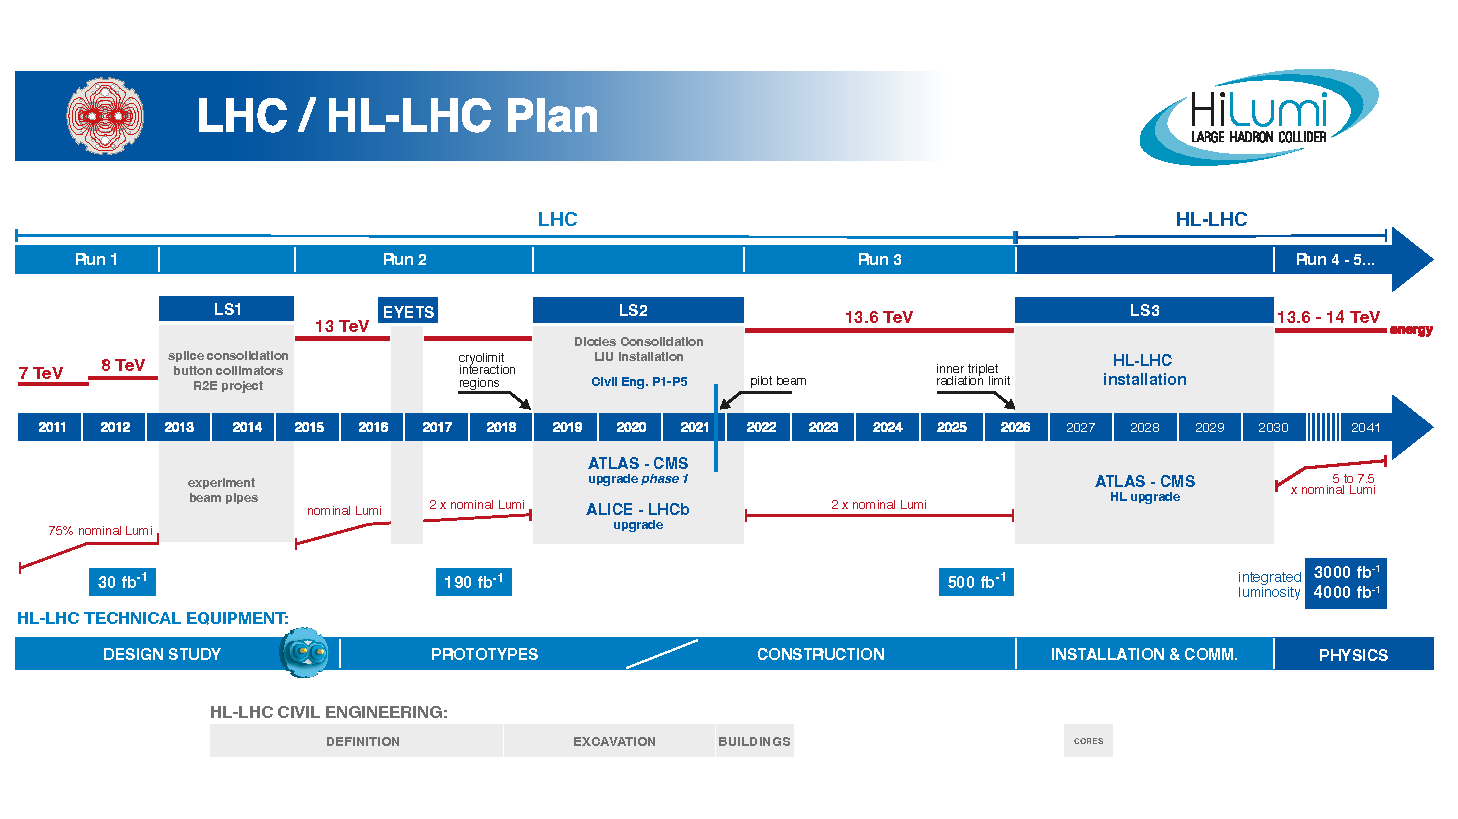
\includegraphics[width=\linewidth]{fig/lhc_hl_lhc.pdf}
\caption[Caption]{\label{fig:lhc:hl_lhc}Caption \citep{lhc:hl_lhc}}
\end{center}
\end{figure}

\subsubsection*{Physics at the LHC}

\begin{figure}[!htbp]
\begin{center}
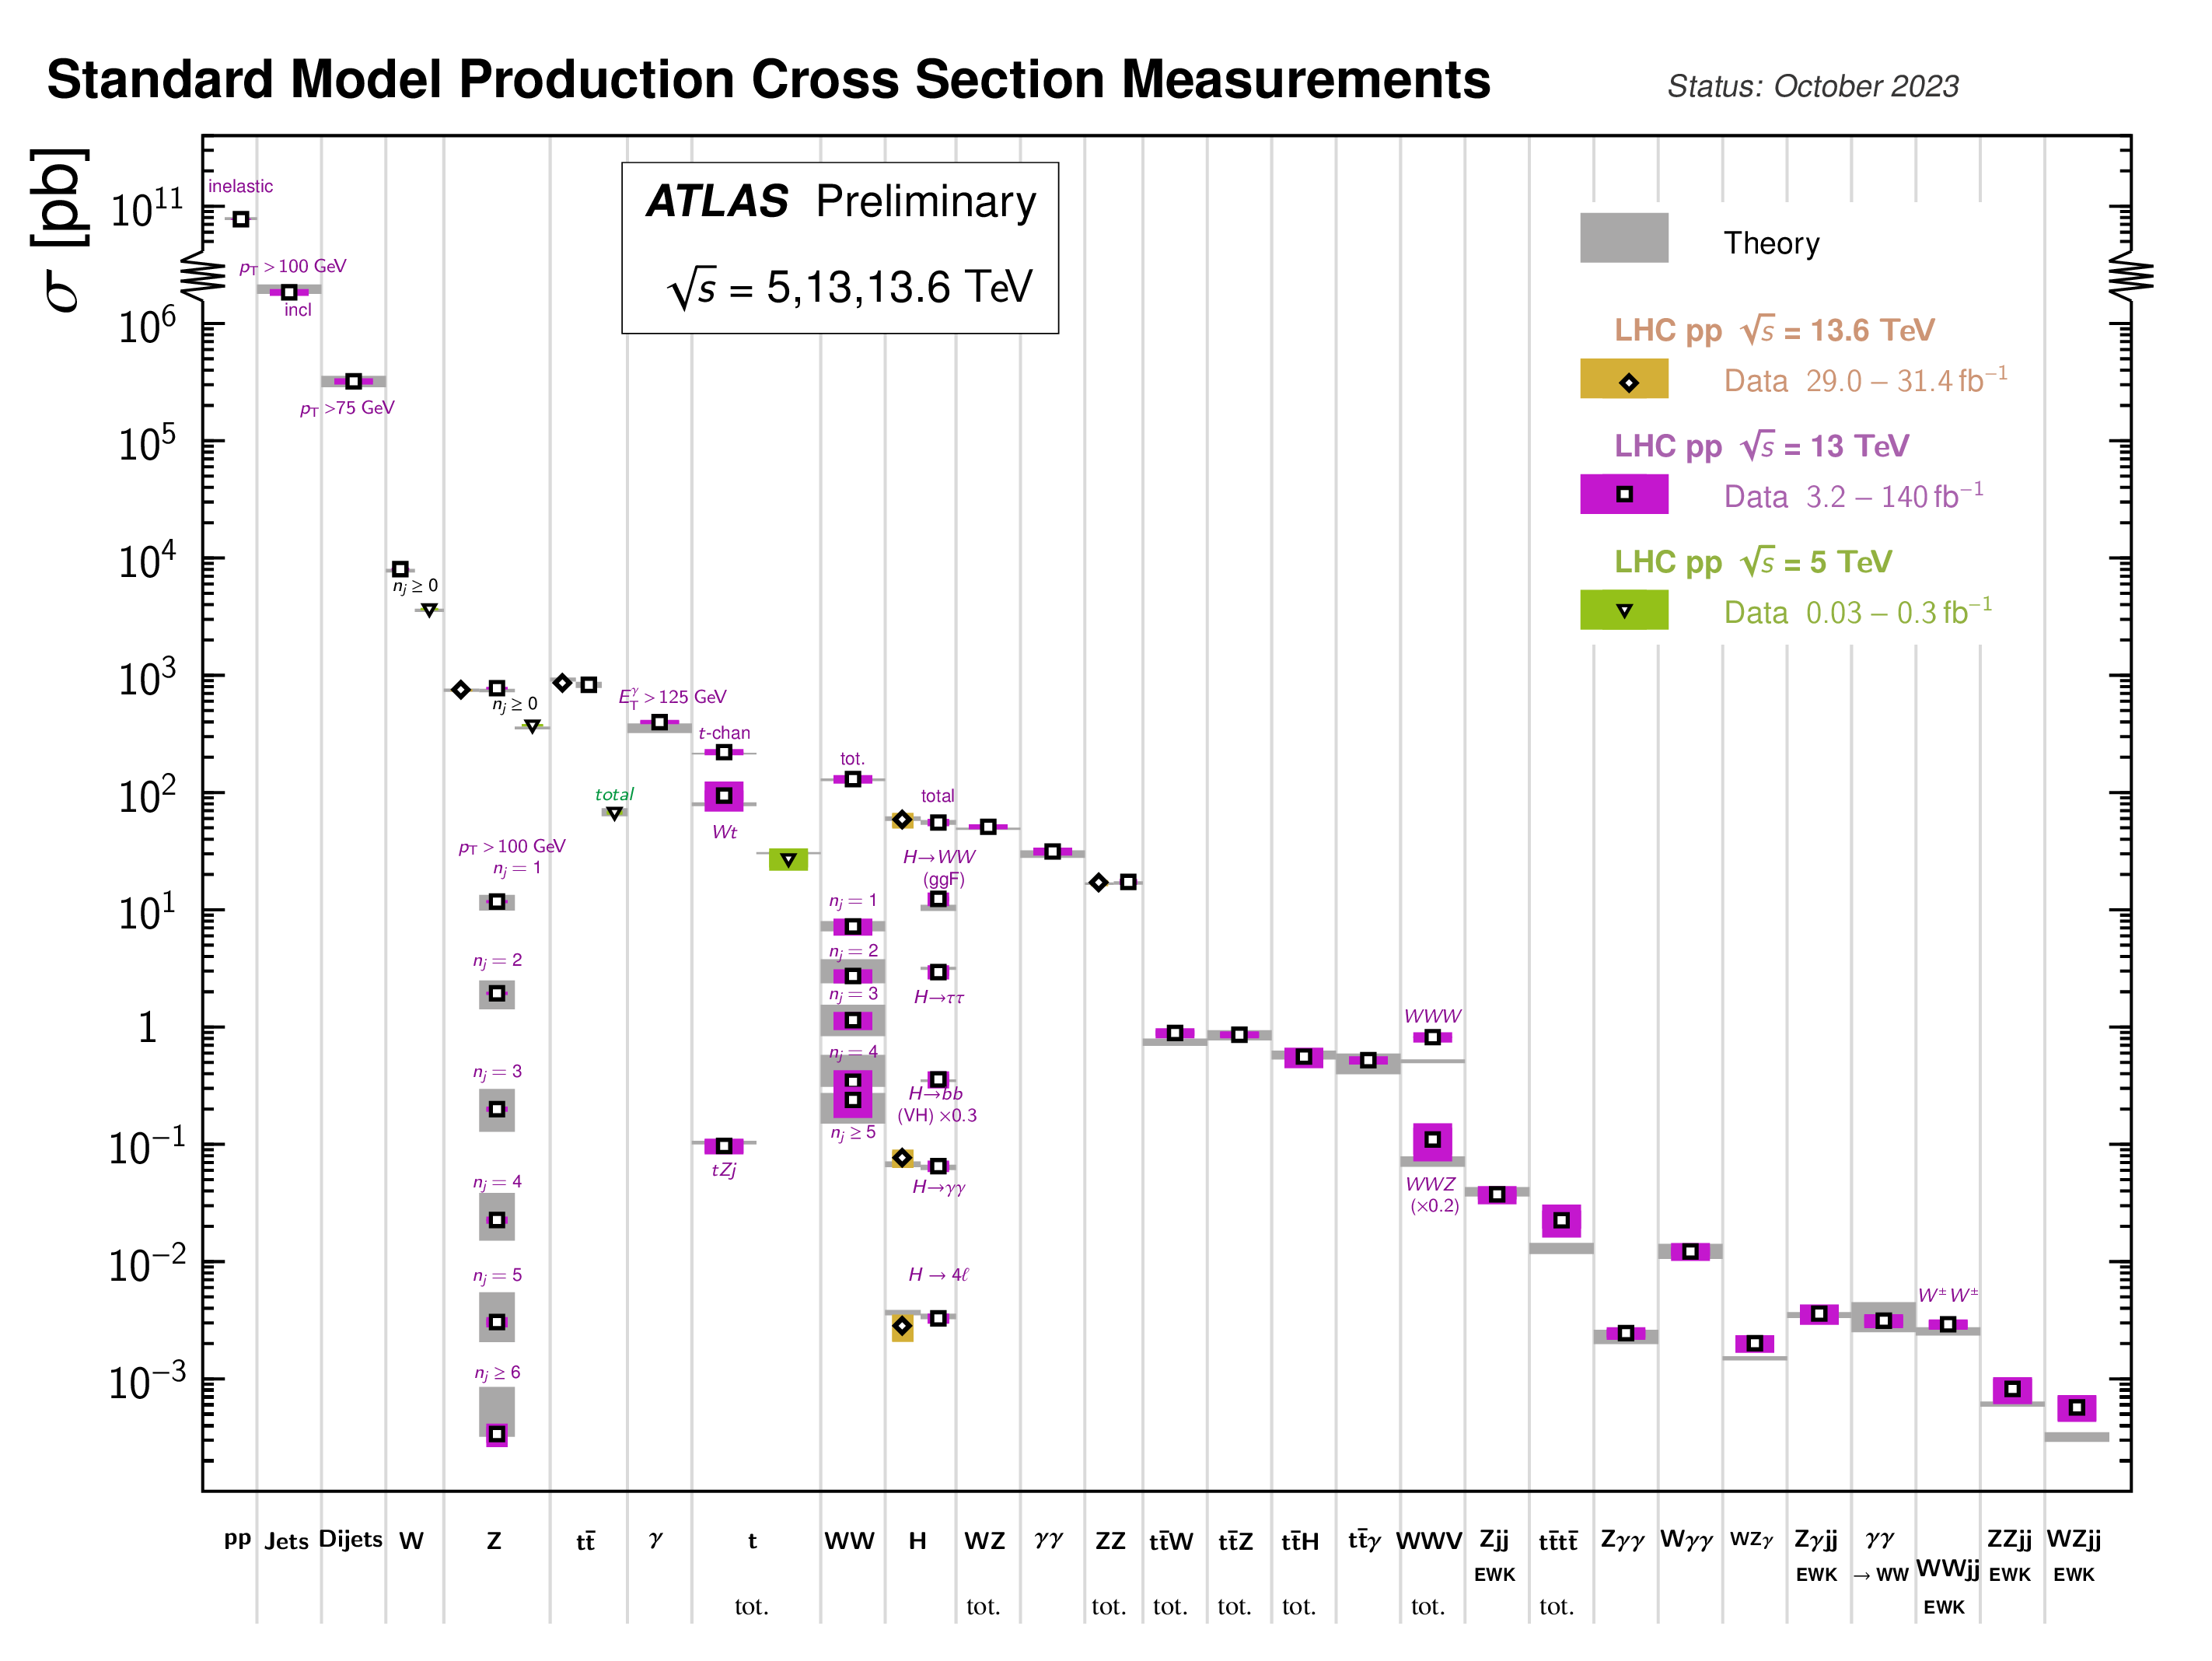
\includegraphics[width=\linewidth]{fig/lhc_xsec_Run23.png}
\caption[Caption]{\label{fig:lhc:xsec}Caption \citep{ATL-PHYS-PUB-2023-039}}
\end{center}
\end{figure}


\section{The ATLAS detector}
\label{sec:ATLAS}
multipurpose particle detector with a symmetric cylindrical geometry and a solid angle coverage of almost $4\pi$\\
44m long, 25m diameter\\
inner detector, solenoid/toroid magnet, EM \& hadronic calorimeters, muon spectrometer\\
(insert figure)


right-handed cylindrical system, z-axis follows beamline, azimuthal and polar (0 in the beam direction) angles measured with respect to beam axis.\\
pseudorapidity $\eta = -\ln \tan (\theta/2)$, approaches $\pm\inf$ along and 0 orthogonal to the beamline\\
distance $\Delta R=\sqrt{\Delta \eta^2 + \Delta \phi^2}$\\
transverse energy $E_\text{T}=\sqrt{\pT ^2+m^2}$\\
transverse momentum \pT component of momentum orthogonal to the beam axis $\pT = \sqrt{p_x^2 + p_y^2}$

\subsection{Inner detector}
\begin{itemize}
\item measures tracks of charged particles with high momentum resolution ($\sigma_{\pT} / \pT = 0.05\% \pm 1\%$
\item covers particles with $\pT>0.5 \text{ GeV}$, $|\eta| < 2.5$\\
pixel detector -> semiconductor tracker -> transition radiation tracker, innermost to outermost
\item pixel detector:
\begin{itemize}
\item innermost, 250 \textmu m silicon pixel layers
\item detects charged particles from electron-hole pair production in silicon
\item measures impact parameter resolution \& vertex identification for reconstruction of short-lived particles
\item spatial resolution of 10 \textmu m in the $R-\phi$ plane and 115 \textmu m in the z-direction
\item 80.4m readout channels
\end{itemize} 
\item sct:
\begin{itemize}
\item surrounds pixel detector, silicon microstrip layers with 80 \textmu m strip pitch
\item particle tracks cross 8 strip layers
\item measures particle momentum, impact parameters, vertex position
\item spatial resolution of 17 \textmu m in the $R-\phi$ plane and 580 \textmu m in the z-direction
\item 6.3m readout channels.
\end{itemize}
\item trt:
\begin{itemize}
\item outermost, layers of 4 mm diameter gaseous straw tubes with transition radiation material (70\% $Xe$ + 27\% $CO_2$ + 3\% $O_2$) \& 30 \textmu m gold-plated wire in the center
\item tubes 144 cm length in barrel region ($|\eta|<1$), 37 cm in the endcap region ($1<|\eta|<2$), arranged in wheels instead of parallel to beamline)
\item gas mixture produces transition radiation when ionized for electron identification
\item resolution/accuracty of 130 \textmu m for each straw tube in the $R-\phi$ plane
\item 351k readout channels
\end{itemize}
\end{itemize}


\subsection{Calorimeter systems}
surrounds the inner detector \& solenoid magnet, covers $|\eta|<4.9$ and full $\phi$ range. Alternates passive and active material layers. Incoming particles passing through calorimeter produce EM cascades or hadronic showers in passive layer. Energies deposited and convert to electric signals in active layers for readout.

\begin{figure}[!htbp]
\begin{center}
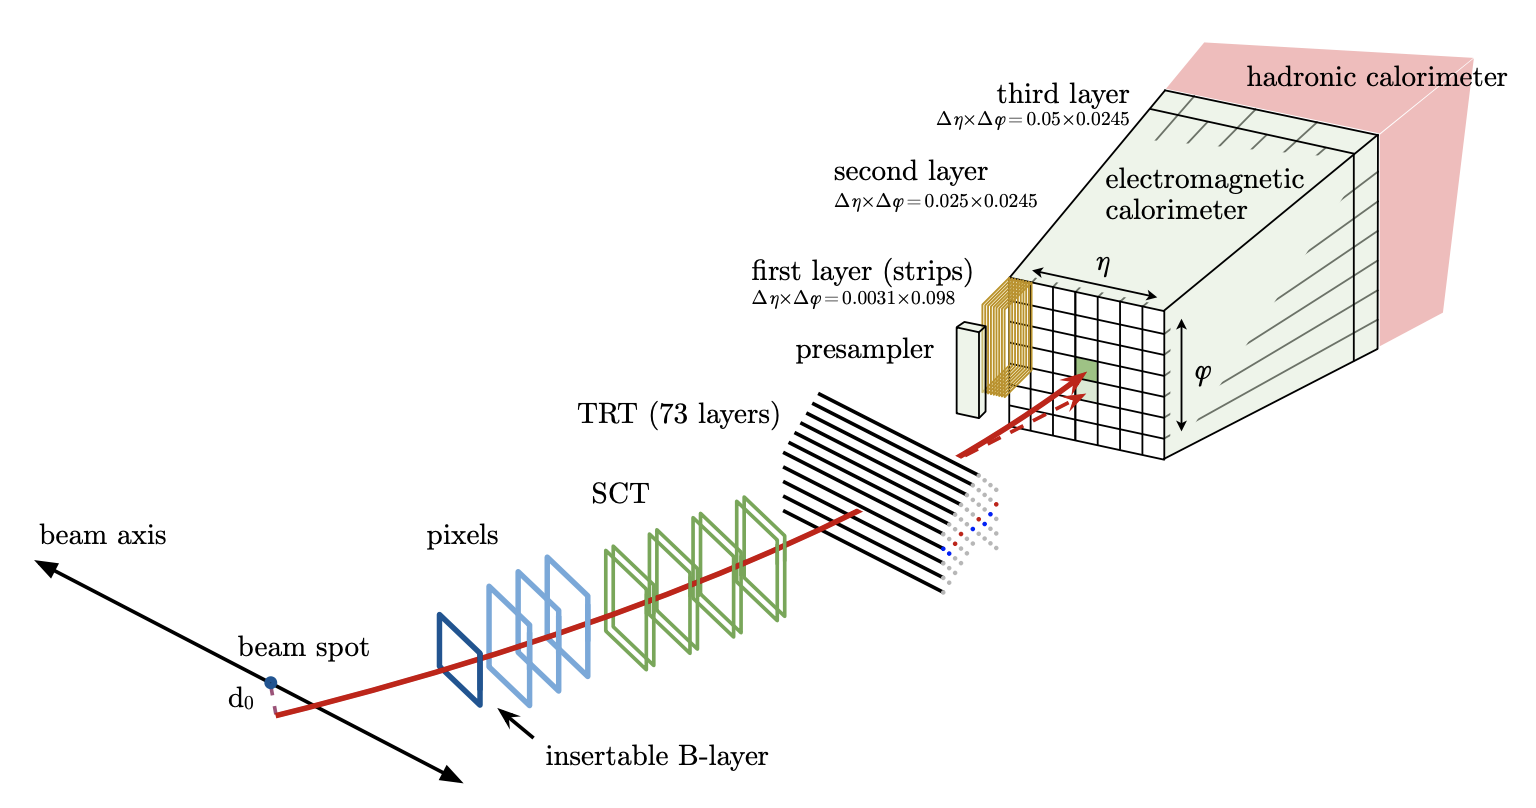
\includegraphics[width=\linewidth]{fig/reco_electron.png}
\caption[Caption]{\label{fig:reco:electron}Caption \citep{reco:electron_id}}
\end{center}
\end{figure}

\begin{multicols}{2}
EM calorimeter: 
\begin{itemize}
\item innermost, lead-LAr detector (passive-active)
\item measures EM cascades (bremsstrahlung \& pair production) produced by electrons/photons
\item divided into barrel region ($|\eta|<1.475$) \& endcap regions ($1.375<|\eta|<3.2$) with transition region ($1.372<|\eta|<1.52$) containing extra cooling materials for inner detector
\item end-cap divided into outer wheel ($1.372<|\eta|<2.5$) \& inner wheel ($2.5<|\eta|<3.2$)
\item higher granularity in ID ($|\eta|<2.5$) range for electrons/photons \& precision physics, coarser elsewhere for jet reconstruction \& MET measurements
\end{itemize}

%\columnbreak
hadronic calorimeter: 
\begin{itemize}
\item outermost
\item measures hadronic showers from inelastic QCD collisions
\item thick enough to prevent most particles showers from reaching muon spectrometer
\item split into tile calorimeter in barrel region ($|\eta|<1.0$) \& extended barrel region ($0.8<|\eta|<1.7$), LAr hadronic end-cap calorimeter (HEC) in end-cap regions ($1.5<|\eta|<3.2$)  \& LAr forward calorimeters (FCal) in $3.1<|\eta|<4.9$ range.

\begin{itemize}
\item tile calorimeters: steel-plastic scintillating tiles, readout via photomultiplier tubes
\item hec: behind tile calorimeters, 2 wheels per end-cap. copper plates-LAr. overlap with other calorimeter systems to cover for gaps between subsystems
\item fcal: 1 copper module \& 2 tungsten modules-LAr. copper optimized for EM measurements, tungsten for hadronic.
\end{itemize}
\end{itemize}
\end{multicols}

\subsection{Muon spectrometer}
\begin{itemize}
\item ATLAS outermost layer. measures muon momenta \& charge in range $|\eta|<2.7$
\item momentum measured by deflection in track from toroid magnets producing magnetic field orthogonal to muon trajectory
\begin{itemize}
\item large barrel toroids in $|\eta|<1.4$, strength 0.5 T
\item 2 smaller end-cap toroids in $1.6<|\eta|<2.7$, strength 1 T
\item transition region $1.4<|\eta|<1.6$, deflection provided by a combination of barrel and end-cap magnets
\end{itemize}
\item chambers installed in 3 cylindrical layers, around the beam axis in barrel region \& in planes perpendicular to beam axis in the transition and end-cap regions
\item split into high-precision tracking chambers (monitored drift tubes \& cathode strip chambers) \& trigger chambers (resistive plate chambers \& thin gap chambers)
\item trigger chambers provide fast muon multiplicity \& approximate energy range information with L1 trigger logic
\begin{multicols}{2}
\begin{itemize}
\item mdt:
	\begin{itemize}
	\item range $|\eta|<2.7$, innermost layer $|\eta|<2.0$
	\item precision momentum measurement
	\item layers of 30 mm drift tubes filled with 93\% $Ar$ \& 7\% $CO_2$, with a 50 \textmu m gold-plated tungsten-rhenium wire at the center
	\item muons pass through tube, ionizing gas and providing signals. Combining signals from tubes forms track
	\item maximumn drift time from wall to wire ~700 ns
	\item resolution: 35 \textmu m per chamber, 80 \textmu m per tube
	\end{itemize}
\item csc:
	\begin{itemize}
	\item forward region $2.0<|\eta|<2.7$, highest particle flux and density region
	\item multiwire proportional chambers with higher granularity, filled with 80\% $Ar$ \& 20\% $CO_2$
	\item shorter drift time than MDT, plus other features making CSC suitable for high particle densities and consequently able to handle background conditions
	\item resolution: 40 \textmu m in bending $\eta$-plane, 5 mm in nonbending $\phi$-plane due to coarser cathode segmentation, per CSC plane
	\end{itemize}
	
\columnbreak
\item rpc:
	\begin{itemize}
	\item range $|\eta|<1.05$
	\item provide fast meas
	\end{itemize}
\item tgc:
	\begin{itemize}
	\item range $1.05<|\eta|<2.7$
	\end{itemize}
\end{itemize}
\end{multicols}
\end{itemize}

\subsection{Forward detectors}
\begin{itemize}
\item LUCID (LUminosity measurement using Cherenkov Integrating Detector): $\pm 17$ m from interaction point, measures luminosity using $pp$ scattering in the forward region
\item ALFA (Absolute Luminosity for ATLAS): $\pm 240$ m, measures $pp$ scattering at small angles
\item ZDC (Zero-Degree Calorimeter): $\pm 140$ m, measures centrality in heavy-ion collisions
\end{itemize}

\subsection{Magnetic systems}
superconducting solenoid \& toroid magnets cooled to 4.5 K with liquid helium\\
solenoid: 2.56 m diameter, 5.8 m length, 2 T strength axial magnetic field, encloses inner detector\\
toroid = barrel + endcap toroid x2\\
barrel toroid: 9.2/20.1 m inner/outer diameter, 25.3 m length, 0.5 T strength\\
endcap toroid: 1.65/10.7 m inner/outer diameter, 5 m length, 1 T strength\\
(show magnet system diagram)

\subsection{Trigger \& data acquisition}
LHC produces large amount of data (40 MHz with 25 ns bunch crossing), necessitates a way to filter out trash from interesting events\\
handles online processing, selecting and recording interesting events for further offline processing and more in-depth analyses\\
\begin{itemize}
\item Level-1 (L1) trigger: online, fast hardware-based trigger, reduces to 100 kHz
\begin{itemize}
\item L1 calorimeter triggers (L1Calo): selects high energy objects \& MET
\item L1 muon triggers (L1Muon): selects using hit information from RPC \& TGC
\item L1 topological trigger (L1Topo): select based on topological selection synthesized using information from L1Calo \& L1Muon
\item Central Trigger Processor (CTP): uses L1Calo/Muon/Topo for final L1 trigger decision within $2.5 \text{ $\mu$s}$ latency. Also identify regions of interest in $\eta$ and $\phi$ to be processed directly by HLT
\end{itemize}
\item L1 trigger information read out by Front-End (FE) detector electronics then sent to ReadOut Drivers (ROD) for preprocessing and subsequently to ReadOut System (ROS) to buffer
\item High-Level Trigger (HLT): offline, software-based trigger, using dedicated algorithms and L1 output as input, reduces to 1 kHz
\item Send to storage for analyses after HLT
\end{itemize}
overall trigger process reduces original collision data rate by a factor of about 10000 after HLT\\
(show TDAQ diagram)





\end{document}